\chapter[The Product of Exponentials Formula]{The Product of Exponentials\\Formula}
\label{ch:poe}

The golfer's joint configuration determines where a rigid club model places its face. It does not determine the muscle forces that produced that configuration, and it does not by itself determine the face velocity. Those require additional maps and state variables. Forward kinematics is the first link in that chain of reasoning: a declared geometry maps joint coordinates to a tool pose. Differentiating that same map gives the instantaneous motion directions available to the task.

The product of exponentials (PoE) makes this construction systematic. A joint is represented by a screw axis at a reference configuration; its finite displacement is a matrix exponential. Multiplying the displacements in the correct order gives the endpoint pose. The order matters because upstream motion carries downstream axes. A consistent derivation also produces the Jacobian, its force dual and the local equations used in inverse kinematics. Each result must retain the same frame, point, coordinate ordering and task definition.

\section{Historical Context and the Choice of Representation}
\label{sec:poe_history}
\label{laymans:context_box}

Denavit--Hartenberg (D-H) parameters and PoE are alternative descriptions of serial-chain geometry, not competing laws of motion. The original D-H construction provides a systematic relationship between neighboring link frames~\cite{dh1955}. Murray, Li and Sastry and Lynch and Park develop Lie-group and screw-based kinematics~\cite{Murray1994,Lynch2017}. Both approaches remain useful; neither removes the need to calibrate axes, choose coordinate signs or define the tool.

D-H frame assignment can be nonunique, especially for parallel or coincident axes. This is a parameterization issue, not proof that the physical robot is singular. PoE can simplify those assignments by storing joint axes in one reference frame. Its numerical matrices still depend on that frame. ``Coordinate-free'' should not be used to imply that recorded screw coordinates are absolute physical quantities.

\subsection{A Common Contract Before Calculation}

Assume an open serial chain of rigid links with ideal one-degree-of-freedom revolute, prismatic or constant-pitch helical joints. Number joints from base to tool. The base frame is fixed for this calculation. Joint coordinates $q_i$ are displacements from a declared home state; they need not be motor-shaft readings when gearing or transmission compliance intervenes. Revolute/helical coordinates use radians; prismatic coordinates use length.

Let $T(q)=T_{sb}(q)$ map homogeneous coordinates from tool frame $\{b\}$ into base frame $\{s\}$. Write
\begin{equation}
 T=\begin{bmatrix}R&p\\0^T&1\end{bmatrix},\qquad
 R\in SO(3),\quad p\in\mathbb R^3,\qquad M=T(0).
\end{equation}
$M$ is the tool's home pose, not the base frame itself. A constant tool offset changes $M$ and the point of interest. Closed chains, floating bases and deformation require the extensions discussed below; a larger joint count alone does not make those assumptions disappear.

\section{Screws and Twists: A Geometric Foundation}
\label{sec:screw_foundation}

Use angular-first six-vectors throughout:
\begin{equation}
 S_i=\begin{bmatrix}\omega_i\\v_i\end{bmatrix},\qquad
 [S_i]=\begin{bmatrix}[\omega_i]_\times&v_i\\0^T&0\end{bmatrix},
 \qquad [\omega]_\times x=\omega\times x.
\end{equation}
The six-vector is a coordinate representation; its bracketed $4\times4$ matrix belongs to $\mathfrak{se}(3)$. Only the upper-left $3\times3$ block is skew-symmetric. The complete matrix generally is not, because its translation column has no matching negative bottom row.

For a revolute axis through home point $r_i$ with unit direction $\omega_i$,
\begin{equation}
 v_i=-\omega_i\times r_i.
\end{equation}
Adding a multiple of $\omega_i$ to $r_i$ leaves the same axis. A helical joint with signed pitch $h_i$ instead has $v_i=-\omega_i\times r_i+h_i\omega_i$. For a prismatic joint, $\omega_i=0$ and $v_i$ is the unit translation direction. These normalization conventions assign the physical displacement scale to $q_i$.

The exponential $E_i(q_i)=\exp([S_i]q_i)$ is a rigid displacement. For a revolute joint its rotation is $R_i=\exp([\omega_i]_\times q_i)$ and its translation is $(I-R_i)r_i$. A rotation about an offset line can therefore have a nonzero translation column without being a screw of nonzero pitch. An axis through the origin has zero translation column for pure rotation.

\section[The Forward Kinematics Equation: Space-Frame PoE]{The Forward Kinematics Equation:\\Space-Frame PoE}
\label{sec:poe_formula}
\begin{equation}
 \label{eq:poe_space_frame}
 T(q)=E_1(q_1)E_2(q_2)\cdots E_n(q_n)M.
\end{equation}
The stored $S_i$ are all expressed in the base frame at home. They are constant model parameters. The current base-frame axis of joint $i$ is generally different: upstream joints carry it through space.

\subsection{Derivation From First Principles}
\label{subsec:poe_derivation}

One derivation sets the most distal joint first, then works toward the base. Joint $n$ moves the tool to $E_nM$. Moving joint $n-1$ next carries that entire downstream assembly, giving $E_{n-1}E_nM$. Continuing toward joint 1 gives Equation~\ref{eq:poe_space_frame}. This is a construction of a configuration, not a requirement that a golfer activate joints in that temporal order.

An equally useful derivation starts proximally. After moving joint 1, joint 2's current generator is $E_1[S_2]E_1^{-1}$. Its displacement about that moved axis is
\begin{equation}
 \exp(E_1[S_2]E_1^{-1}q_2)=E_1E_2E_1^{-1}.
\end{equation}
Applying it to $E_1M$ gives $E_1E_2M$, not $E_2E_1M$. The conjugations account for the transported axis. More generally, with prefix $P_{i-1}=E_1\cdots E_{i-1}$, the current spatial screw is $\operatorname{Ad}_{P_{i-1}}S_i$.

Matrix action on a column vector proceeds from right to left. Joint numbering in a written product and the order of a hypothetical sequence of isolated moves are different descriptions. The formula must be checked algebraically rather than justified by saying simply that a joint ``acts first.''

\begin{figure}[htbp]
\centering
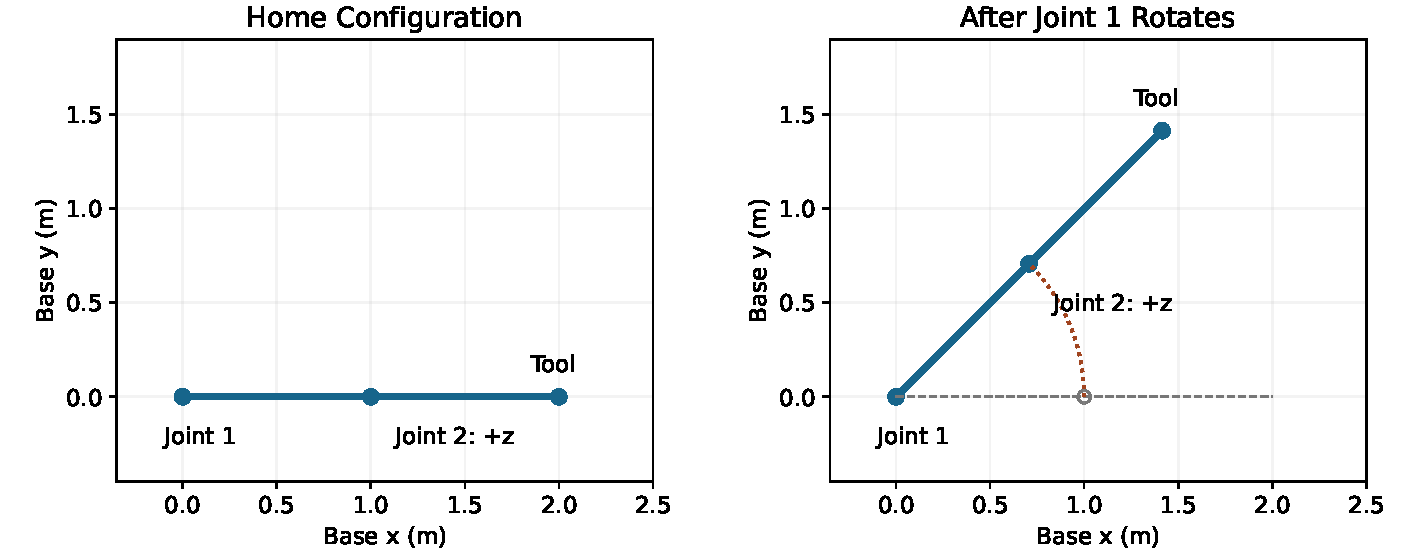
\includegraphics[width=\linewidth]{../figures/poe_transported_axis.pdf}
\caption{An Upstream Rotation Carries the Downstream Axis. The Home Axis Is a Constant Model Parameter; the Current Axis Passes Through the Moved Elbow.}
\label{fig:product_exponentials}
\end{figure}

\section{Body-Frame PoE: Motion Relative to the Tool}
\label{sec:body_frame_poe}
\label{subsec:poe_conversion}

Define constant home axes in the home tool frame by
\begin{equation}
 B_i=\operatorname{Ad}_{M^{-1}}S_i,\qquad
 \label{eq:adjoint_conversion}
 S_i=\operatorname{Ad}_M B_i.
\end{equation}
For an angular-first twist and $T=(R,p)$,
\begin{equation}
 \operatorname{Ad}_T=
 \begin{bmatrix}R&0\\{[p]_\times R}&R\end{bmatrix},\qquad
 [\operatorname{Ad}_T V]=T[V]T^{-1}.
\end{equation}
Because $[B_i]=M^{-1}[S_i]M$, each $E_i=M\exp([B_i]q_i)M^{-1}$. Substituting these factors causes adjacent $M^{-1}M$ pairs to cancel:
\begin{equation}
 \label{eq:poe_body_frame}
 T(q)=M\exp([B_1]q_1)\exp([B_2]q_2)\cdots\exp([B_n]q_n).
\end{equation}
The joint index order is still $1,\ldots,n$. The home transform changes sides; the order does not reverse. Converting the constant home axes uses $M$. Converting current velocity representations uses $T(q)$ instead. Substituting a current pose into a home-axis definition silently changes the model.

\section{Velocity Kinematics and the Spatial Jacobian}
\label{sec:spatial_jacobian}
\label{sec:velocity_kinematics}

Define spatial and body twist matrices by
\begin{equation}
 [V_s]=\dot T T^{-1},\qquad [V_b]=T^{-1}\dot T.
\end{equation}
The bracket notation matters: neither matrix is itself a six-vector. For $T=(R,p)$,
\begin{equation}
 [\omega_s]_\times=\dot R R^T,\qquad
 v_s=\dot p-\omega_s\times p,\qquad
 \dot p=v_s+\omega_s\times p.
\end{equation}
Thus the linear part of the spatial twist is generally not the velocity of the tool origin. In body coordinates, $\omega_b=R^T\omega_s$ and $v_b=R^T\dot p$. A force or velocity calculation that mixes these meanings can be dimensionally plausible but physically wrong.

For a constant generator $A$, $d\exp(Aq(t))/dt=A\exp(Aq)\dot q$. The factor is $A\dot q$, not $Aq$, and a general time-dependent matrix requires a more careful derivative if it does not commute with its derivative. The product rule gives
\begin{equation}
 \dot T=\sum_{i=1}^n P_{i-1}[S_i]E_i\cdots E_nM\,\dot q_i.
\end{equation}
Right-multiplication by $T^{-1}$ cancels every factor after $[S_i]$, yielding
\begin{equation}
 [V_s]=\sum_{i=1}^n P_{i-1}[S_i]P_{i-1}^{-1}\dot q_i.
\end{equation}
Taking six-vector coordinates gives
\begin{equation}
 \label{eq:spatial_jacobian}
 V_s=J_s(q)\dot q,\qquad
 J_{s,i}=\operatorname{Ad}_{P_{i-1}}S_i,\quad P_0=I.
\end{equation}
The adjoint is $6\times6$. Multiplying a homogeneous $4\times4$ transform directly by a six-vector is undefined. Column $i$ depends only on joints preceding $i$; a prefix recursion computes the full Jacobian without finite differences.

\subsection{Body Jacobian and the Adjoint Relationship}
\label{sec:body_jacobian}
\begin{equation}
 \label{eq:jacobian_adjoint}
 J_b=\operatorname{Ad}_{T^{-1}}J_s,\qquad V_b=J_b\dot q.
\end{equation}
Writing $H_i=\exp([B_i]q_i)$ gives the equivalent suffix formula
\begin{equation}
 J_{b,i}=\operatorname{Ad}_{H_n^{-1}\cdots H_{i+1}^{-1}}B_i.
\end{equation}
This expression depends on the joints after $i$. At home, $J_s(0)$ has columns $S_i$ and $J_b(0)$ has columns $B_i$; these are useful convention checks.

\subsection{Point Velocity and Numerical Verification}
\label{subsec:jacobian_numerical}

For a material point with fixed tool coordinates $c$, its base position is $x=p+Rc$. Its velocity and position Jacobian are
\begin{equation}
 \dot x=\omega_s\times x+v_s,\qquad
 J_x=\begin{bmatrix}-[x]_\times&I\end{bmatrix}J_s.
\end{equation}
Changing the clubface point changes $J_x$. A spatial twist describes the whole rigid body and is independent of the tool-origin choice; a particular point velocity is not.

A central difference provides an independent check:
\begin{equation}
 D_iT\approx\frac{T(q+\epsilon e_i)-T(q-\epsilon e_i)}{2\epsilon},\qquad
 [J_{s,i}]\approx(D_iT)T^{-1}.
\end{equation}
Extract angular coordinates from the skew part of the upper-left block and linear coordinates from the upper-right column. Choose $\epsilon$ in the units of the perturbed coordinate and study convergence; arbitrarily tiny steps amplify roundoff. Automatic differentiation checks the implemented map, which can still represent the wrong geometry. An independent link construction is therefore a stronger ordering test.

\section{Comparison With D-H: A Complete Planar Example}
\label{sec:dh_limitations}
\label{sec:poe_vs_dh}

For the standard D-H convention used here,
\begin{equation}
 A_i=R_z(q_i)\operatorname{Trans}_z(d_i)
       \operatorname{Trans}_x(a_i)R_x(\alpha_i).
\end{equation}
The axis on each translation must be stated. Modified D-H uses a different factor ordering and indexing; its parameter table cannot be substituted into this expression unchanged.

\subsection{D-H Parametrization}
\label{subsec:dh_example}

Take three planar revolute joints with link lengths $(L_1,L_2,L_3)=(1,0.8,0.6)$ m, home links along positive $x$, and positive rotations about $z$. Choose $a_i=L_i$, $d_i=\alpha_i=0$. Then
\begin{equation}
 T=A_1A_2A_3,\qquad A_i=R_z(q_i)\operatorname{Trans}_x(L_i).
\end{equation}
This includes all three links. A different frame assignment may instead leave a final fixed tool transform, but that transform must be included before claiming equivalence.

\subsection{PoE Parametrization and Independent Evaluation}
\label{subsec:poe_example}

Here $M$ is identity orientation with $p_0=(2.4,0,0)^T$, and
\begin{equation}
 S_1=(0,0,1,0,0,0)^T,\quad
 S_2=(0,0,1,0,-1,0)^T,\quad
 S_3=(0,0,1,0,-1.8,0)^T.
\end{equation}
PoE and the declared D-H product both give orientation $R_z(q_1+q_2+q_3)$ and
\begin{equation}
 p=\sum_{i=1}^3 L_i
 \begin{bmatrix}\cos(q_1+\cdots+q_i)\\\sin(q_1+\cdots+q_i)\\0\end{bmatrix}.
\end{equation}
At $(45,-30,60)$ degrees, the yaw is $75$ degrees and $p=(1.635139,1.493718,0)^T$ m. This explicit endpoint formula tests the matrix implementation independently. Agreement is not guaranteed by naming two routines ``D-H'' and ``PoE''; both must encode the same frames and terminal link.

\subsection{Computational Advantages and Limits}
\label{subsec:poe_advantages}

PoE stores the home pose and axes directly and produces an economical prefix Jacobian recursion. D-H can be compact when a mechanism already has a verified parameter table. Computational speed depends on the implementation, sparsity and required outputs; neither notation supplies a universal speed advantage. Uncertainty in an axis location, an encoder zero or a fixed tool offset propagates into both formulations.

\section{Prismatic Joints and Mixed Chains}
\label{sec:prismatic_joints}

For unit direction $d$ and translation coordinate $s$,
\begin{equation}
 S=(0,d)^T,\qquad
 \exp([S]s)=\begin{bmatrix}I&sd\\0^T&1\end{bmatrix}.
\end{equation}
The same ordered PoE formula handles a revolute-prismatic chain. An upstream rotation carries a downstream prismatic direction, so its current direction cannot generally be kept fixed in world coordinates.

\subsection{Example: Cartesian Translation}
\label{subsec:cartesian_example}

For three mutually orthogonal prismatic axes, $S_x=(0,e_x)^T$, $S_y=(0,e_y)^T$, $S_z=(0,e_z)^T$ and $M=I$, the product has $R=I$ and $p=(s_x,s_y,s_z)^T$. Pure translations commute, so reversing these particular factors does not reveal an ordering bug. A rotation/translation or nonparallel-rotation example is essential in a test suite. The spatial Jacobian is $[0;I]$, with rank three; this mechanism is not singular everywhere merely because it cannot control all six pose directions.

\section{Worked Example: A Spatial 3R Robot}
\label{sec:worked_example_3r}

Use a $z$-axis joint at the origin, a $y$-axis joint through $(0.5,0,0)$ m at home, and an $x$-axis joint through $(0.8,0,0)$ m at home. The three home links have lengths $0.5$, $0.3$ and $0.2$ m along $x$. This is a declared teaching mechanism, not an anatomical fit.

\subsection{Home Pose and Screw Axes}
\label{subsec:home_config}
\label{subsec:spatial_screw_axes}
\begin{equation}
 M=\begin{bmatrix}I&(1,0,0)^T\\0^T&1\end{bmatrix},\qquad
 \begin{aligned}
 S_1&=(0,0,1,0,0,0)^T,\\
 S_2&=(0,1,0,0,0,0.5)^T,\\
 S_3&=(1,0,0,0,0,0)^T.
 \end{aligned}
\end{equation}
The third axis lies along the entire home $x$ line, which also passes through the origin. Its zero linear component is therefore correct. Rotating it changes tool orientation while leaving the tool origin on that axis. This distinction will reappear in task-dependent rank.

\subsection{Numerical Evaluation at a Test Configuration}
\label{subsec:spatial_3r_eval}

At $q=(\pi/4,\pi/6,-\pi/3)$, the second factor is
\begin{equation}
 E_2\approx\begin{bmatrix}
 0.866025&0&0.5&0.066987\\
 0&1&0&0\\
 -0.5&0&0.866025&0.25\\
 0&0&0&1
 \end{bmatrix}.
\end{equation}
Its translation is $(I-R_y(\pi/6))(0.5,0,0)^T$. The third factor is a pure $x$ rotation with no translation. The complete result is
\begin{equation}
 T\approx\begin{bmatrix}
 0.612372&-0.659740&-0.435596&0.659740\\
 0.612372&0.047367&0.789149&0.659740\\
 -0.5&-0.75&0.433013&-0.25\\
 0&0&0&1
 \end{bmatrix}.
\end{equation}
An independent link construction gives $R=R_z(q_1)R_y(q_2)R_x(q_3)$ and
\begin{equation}
 p=R_z(q_1)\left[
 \begin{pmatrix}0.5\\0\\0\end{pmatrix}
 +R_y(q_2)\begin{pmatrix}0.5\\0\\0\end{pmatrix}\right].
\end{equation}
It agrees with PoE. In particular, $p$ is independent of $q_3$, although $R$ is not. This is a geometric property of this axis/tool choice, not an error or an inability of the third joint to act.

\section{Singularities Belong to a Declared Task}
\label{sec:singularities}
\label{subsec:singularity_types}

Let $y=h(q)$ be the selected task and $J_y=Dh(q)$. A singular configuration is one where its rank drops below the maximum attained for that mechanism and task on the region being considered. A full spatial Jacobian has at most $\min(6,n)$ rank, but the mechanism may have a smaller generic rank. A redundant $6\times7$ Jacobian can have full row rank six while always satisfying $\operatorname{rank}J<7$. That inequality alone therefore cannot define singularity.

At a configuration with rank $r$, attainable instantaneous task velocities lie in $\operatorname{range}J_y$. A desired velocity outside that range has no exact joint-rate solution. The null space has dimension $n-r$. Neither fact by itself proves a loss of nonlinear controllability over time, a physically locked joint, or inability to reach another pose after reconfiguration.

\subsection{A Two-Link Counterexample to Task Conflation}

For a planar 2R arm, the position task $y=(x,y)$ has
\begin{equation}
 J_p=\begin{bmatrix}
 -L_1\sin q_1-L_2\sin(q_1+q_2)&-L_2\sin(q_1+q_2)\\
 L_1\cos q_1+L_2\cos(q_1+q_2)&L_2\cos(q_1+q_2)
 \end{bmatrix},\qquad
 \det J_p=L_1L_2\sin q_2.
\end{equation}
For positive lengths, straight or folded links give rank one instead of the generic rank two. The full spatial twist Jacobian, however, has columns
\begin{equation}
 J_s=\begin{bmatrix}
 0&0\\0&0\\1&1\\0&L_1\sin q_1\\0&-L_1\cos q_1\\0&0
 \end{bmatrix}.
\end{equation}
These columns remain independent for $L_1>0$, including straight configurations. The map to planar pose is an immersion of a two-dimensional joint space into a three-dimensional pose space; it still has only two independent inputs. Losing a direction after projecting to endpoint position does not imply that this full pose map also loses rank.

In golf, a configuration may be favorable for one face-point velocity and unfavorable for changing face orientation or maintaining hand contact. Specify the task before interpreting a singularity or claiming that an extra degree of freedom is unused.

\subsection{Detection and Damped Inversion}
\label{subsec:singularity_handling}

Use singular values of a meaningfully scaled Jacobian. A determinant is a product, not a condition number. For a full-row-rank $m\times n$ map, $\det(JJ^T)$ is the product of its $m$ squared singular values, whereas $\kappa_2(J)=\sigma_{\max}/\sigma_{\min}$. For $n>m$, $\det(J^TJ)=0$ even at every regular full-row-rank configuration. For $m>n$, $\det(JJ^T)=0$ instead. A fixed raw determinant threshold also changes when meters become millimeters.

With consistent scaling, a damped least-squares step is
\begin{equation}
 \Delta q=J^T(JJ^T+\lambda^2 I)^{-1}e,\qquad \lambda>0.
\end{equation}
It minimizes $\|J\Delta q-e\|^2+\lambda^2\|\Delta q\|^2$. In an SVD it uses factors $\sigma_i/(\sigma_i^2+\lambda^2)$, suppressing amplification in weak directions. It deliberately permits task error and does not restore a missing physical direction. Explicit joint limits, collision constraints and a trust region require additional treatment. Rates needed to track a weak direction can grow without bound in an ideal limiting calculation; at the exact singularity, a velocity outside the range is infeasible, rather than a motion achieved by literally infinite joint speed.

\section{Workspace, Manipulability and Force Duality}
\label{sec:workspace_manipulability}
\index{workspace analysis}\index{manipulability}\index{manipulability measure}
\label{def:reachable_workspace}\index{reachable workspace}

Given admissible joint set $\mathcal Q$, the reachable pose set is
\begin{equation}
 \label{eq:reachable_workspace}
 \mathcal W_{\rm pose}=\{T(q):q\in\mathcal Q\}.
\end{equation}
Its projection onto position is a different workspace. A dexterous position workspace can be defined as the positions for which every orientation in a specified orientation set is attainable. For a planar robot, that set might be all yaw angles; demanding every orientation in $SO(3)$ would be a different, usually impossible requirement. Joint bounds, collisions and closed-chain feasibility change $\mathcal Q$.

\subsection{Declare the Metric Before the Ellipsoid}
\label{def:manipulability}\label{def:velocity_ellipsoid}
\index{Yoshikawa manipulability}\index{SVD!of Jacobian}
\index{manipulability ellipsoid!velocity}

The image of a unit joint-rate ball under $J$ is an ellipsoid, possibly degenerate. But joint rates can mix radians per second and meters per second; pose rates mix angular and linear quantities. Choose positive-definite rate and task metrics $W_q,W_y$. For $\dot q^TW_q\dot q\leq1$, define normalized rates and Jacobian by
\begin{equation}
 \eta=W_q^{1/2}\dot q,\qquad \zeta=W_y^{1/2}\dot y,
 \qquad \widetilde J=W_y^{1/2}JW_q^{-1/2}.
\end{equation}
Then $\zeta=\widetilde J\eta$, and the singular values of $\widetilde J$ give the semiaxes in these normalized coordinates. A characteristic length used to compare rotation with translation is a modeling choice, not a universal property of the robot. Actual box-shaped actuator limits generally map to a polytope rather than this ellipsoid.

For a full-row-rank $m$-dimensional task with identity metrics,
\begin{equation}
 \label{eq:manipulability}
 w(q)=\sqrt{\det(JJ^T)}=\prod_{i=1}^m\sigma_i.
\end{equation}
This is the volume scale factor. The actual ellipsoid volume is the unit $m$-ball volume multiplied by $w$. For a planar task it is $\pi w$. When generic rank is less than $m$, full $m$-dimensional volume is always zero; one may report a clearly named lower-dimensional volume, but must not use zero full volume to classify every configuration as singular. Space/body adjoints preserve rank, but generally not singular values because translation makes them nonorthogonal in an unweighted Euclidean six-vector metric.

\subsection{Static Force Bounds Use the Dual Map}
\label{def:force_ellipsoid}\label{laymans:manipulability_duality}
\index{manipulability ellipsoid!force}

For power-conjugate task force $f$ and task velocity $\dot y$, virtual work gives
\begin{equation}
 \tau=J^Tf,\qquad \tau^T\dot q=f^T\dot y.
\end{equation}
Here $f$ can be defined as the force the actuator system applies to a quasistatic load. The force exerted by that load on the robot has the opposite sign in the equilibrium equation. A six-dimensional spatial wrench uses moment-first order and the same reporting origin as $V_s$; mixing it with a point force or another moment origin breaks the power pairing.

Under identity metrics, the ideal torque ball $\|\tau\|\leq1$ implies
\begin{equation}
 \|J^Tf\|^2=f^TJJ^Tf\leq1.
\end{equation}
If $J$ has full row rank, this set has semiaxes $1/\sigma_i$ along the same task directions as the velocity ellipsoid. With the metrics above, use dual force coordinates $W_y^{-1/2}f$ and $W_q^{-1/2}\tau$ to preserve the pairing. Arbitrary torques need not correspond to a static endpoint load, especially for redundant mechanisms.

At rank loss the ideal force set can be unbounded along $\ker J^T$. That describes a load carried by ideal structural constraints without generalized joint torque, not infinite material strength or a force that an actuator can generate at will. Buckling, joint reaction limits, tendon forces, compliance, balance and contact friction still limit a real body. Dynamic forces also involve inertia and acceleration. The velocity/force tradeoff is therefore a local static result under declared bounds, not a statement that a faster golf swing must be weaker.

\subsection{Numerical Example: The Planar 2R Arm}
\label{ex:manipulability_2r}\index{2R arm!manipulability}

For $L_1=L_2=1$ m and $q_1=0$, at $q_2=\pi/4$ the position Jacobian has singular values approximately $2.07313$ and $0.34108$. Their ratio is about $6.08$, so the velocity ellipse is distinctly elongated, not nearly circular. Its scale factor is $w=\sin(\pi/4)\approx0.70711$. At $q_2=0.1$, the singular values are $2.23339$ and $0.04470$, with $w\approx0.09983$. At $q_2=0$, the radial position direction vanishes to first order. A small finite joint change can still move inward through second-order geometry; local rank is not a complete reachable-set calculation.

\begin{figure}[htbp]
\centering
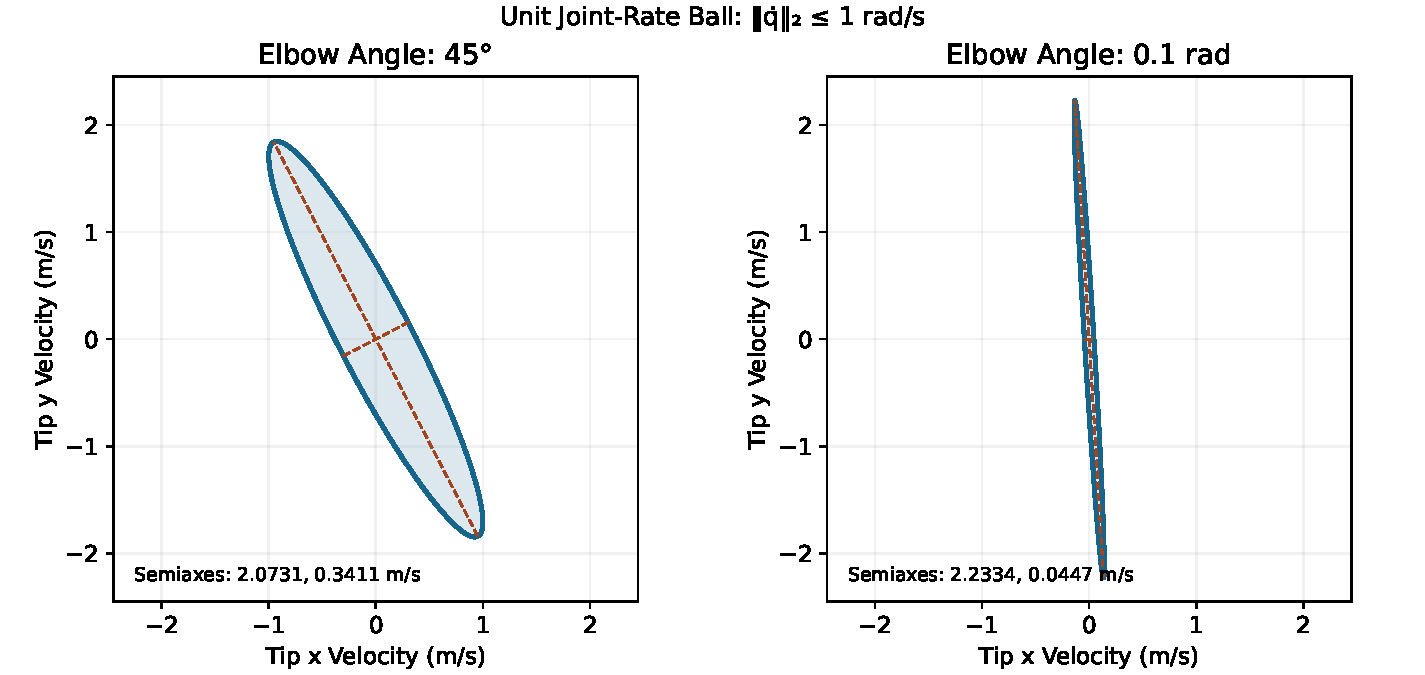
\includegraphics[width=\linewidth]{../figures/poe_velocity_ellipses.pdf}
\caption{Position-Velocity Ellipses for Equal Unit-Length Links. Equal Plot Scales Reveal the Strong Anisotropy Already Present at 45 Degrees and Its Increase Near Extension.}
\label{fig:poe_velocity_ellipses}
\end{figure}

\section{Redundancy and Null-Space Motion}
\label{subsec:null_space_motion}\index{redundancy}\index{null-space motion}
\index{null space!of Jacobian}\index{kinematic redundancy}
\label{def:null_space_projector}\index{null-space projector}

Using the Moore--Penrose inverse defined by the SVD,
\begin{equation}
 \label{eq:null_space_projector}
 N=I-J^\dagger J,\qquad JN=0.
\end{equation}
The shortcut $J^\dagger=J^T(JJ^T)^{-1}$ requires full row rank. The SVD definition remains valid when that shortcut does not. If $\dot y_{\rm des}\in\operatorname{range}J$, all exact solutions are
\begin{equation}
 \label{eq:redundancy_resolution}
 \dot q=J^\dagger\dot y_{\rm des}+Nz.
\end{equation}
Otherwise the first term supplies the least-squares projection of the desired task rate and leaves a residual. A damped inverse generally does not make $I-J^\#J$ an exact null-space projector; a secondary command can then leak into the primary task.

\label{ex:7dof_null_space}\index{7-DOF arm!null-space optimization}
For a regular $6\times7$ pose Jacobian, the null space is one-dimensional. Choosing $z=\alpha\nabla w$, with $\alpha>0$ and a differentiable local objective, gives a nonnegative contribution $\alpha\nabla w^TN\nabla w$ to $\dot w$ for this Euclidean orthogonal projector. The primary task term can still lower $w$; limits or changing rank can obstruct the motion. This is not a guarantee of singularity avoidance or uniformly good force authority.

The null condition is instantaneous. A finite Euler step $q+\Delta q$ with $J\Delta q=0$ generally changes a nonlinear task at order $\|\Delta q\|^2$. Continuous integration with exact recomputation preserves the task only under the stated smoothness and feasibility assumptions. Holding a clubface point fixed also leaves different freedom than holding its complete pose fixed; an internal motion can change grip load or shaft strain even while a chosen task is unchanged.

\section{Inverse Kinematics With a Consistent Pose Error}
\label{sec:inverse_kinematics}

Inverse kinematics asks for $T(q)=T_d$ within the admissible joint set. Some geometries have analytic solutions; general chains often use numerical methods. Multiple solutions, joint bounds and unreachable targets are normal possibilities. A numerical iteration is not a global feasibility certificate.

\subsection{Pose Error Representation}
\label{subsec:pose_error}

A body-frame displacement error is
\begin{equation}
 E=T(q)^{-1}T_d,\qquad e_b=(\log E)^\vee,
\end{equation}
using a specified real $SE(3)$ logarithm branch and angular-first order. It is zero at the desired pose. Applying the vee operator directly to a rotation matrix is invalid: vee in this convention acts on the skew/generator matrix produced by a logarithm. The translation entries of $e_b$ are also coupled to its rotation, and are not generally just $p_d-p$.

Near the target, $T(q+\Delta q)\approx T(q)\exp([J_b\Delta q])$. Hence the local step
\begin{equation}
 \label{subsec:newton_raphson}
 J_b(q)\Delta q\approx e_b
\end{equation}
uses compatible coordinates. Equivalently, transform both sides to the space frame with $\operatorname{Ad}_{T(q)}$. A position-first Euclidean error cannot be inserted unchanged into an angular-first spatial-twist equation.

\subsection{Residual Derivatives and Convergence}

Away from zero error, the exact derivative includes the differential of the logarithm. Let $\mathcal L(e)$ be defined locally by
\begin{equation}
 \log\!\left(\exp([\delta])\exp([e])\right)^\vee
 =e+\mathcal L(e)\delta+O(\|\delta\|^2).
\end{equation}
It is the inverse left Jacobian for this convention, with $\mathcal L(0)=I$. A joint increment left-multiplies $E$ by $\exp(-[J_b\Delta q])$ to first order, giving
\begin{equation}
 De_b=-\mathcal L(e_b)J_b.
\end{equation}
This provides the residual Jacobian for a weighted Newton or least-squares method on a smooth branch. Omitting $\mathcal L$ is a local approximation, not an exact residual derivative at arbitrary error. Near a half-turn, the selected logarithm branch needs special care. A matrix Frobenius residual can also be used as a declared extrinsic objective, but its derivative and units must match that objective.

\subsection{A Practical Local Iteration}
\label{subsec:ik_algorithm}

Choose an initial configuration, task error tolerances and rate/step metrics. At each iteration evaluate the pose, error and consistent Jacobian; solve a bounded or damped local problem; then accept a step only after checking the actual error reduction and feasibility. Stop on separately meaningful angular and position tolerances, or on a declared failure condition such as stagnation or an iteration budget. Record the residual and reason for stopping.

Exact Newton has local quadratic convergence under suitable smoothness, a nonsingular square residual derivative and a sufficiently close initial guess. Redundant, overdetermined, damped or constrained iterations need their own convergence analysis. Failure to converge can result from a poor starting point, a local minimum, an unsuitable branch or step rule, numerical scaling or constraints; it does not prove the target is outside the workspace.

For a position-only planar 2R task, ordinary Cartesian error $p_d-p(q)$ and $J_p$ already form a consistent local pair. With $L_1=1.5$ m, $L_2=1$ m and target $(2,0.5)$ m, one analytic solution is approximately $q=(-0.230011,1.230959)$ rad. The other elbow branch, when admissible, is another solution. Such a direct geometric solution is a useful independent check of a numerical solver.

\section{Python Worked Example}
\label{sec:python_example}

The following self-contained NumPy/SciPy example implements the declared spatial 3R mechanism. It retains angular-first ordering and multiplies each new home-axis exponential on the right of the accumulated prefix. The Jacobian uses analytic adjoint transport. Tests compare the pose with independent link geometry, compare Jacobian columns with central differences and verify point velocity. The demonstration reports the full spatial rank rather than the identically zero determinant of a $6\times6$ Gram matrix for a three-input mechanism.

\begin{lstlisting}[language=Python,basicstyle=\ttfamily\footnotesize,columns=fullflexible,keywordstyle=\color{chapblue},stringstyle=\color{purplehaze},commentstyle=\color{chapblue},numberstyle=\tiny\color{black!65}]
import numpy as np
from scipy.linalg import expm


class SpatialRobot3R:
    """Declared z-y-x serial mechanism; meters and radians."""

    def __init__(self, L1: float = 0.5, L2: float = 0.3,
                 L3: float = 0.2) -> None:
        lengths = np.asarray([L1, L2, L3], dtype=float)
        if not np.isfinite(lengths).all() or np.any(lengths <= 0):
            raise ValueError("Link lengths must be finite and positive")
        self.M = np.eye(4)
        self.M[0, 3] = float(lengths.sum())
        self.axes = np.array([
            [0, 0, 1, 0, 0, 0],
            [0, 1, 0, 0, 0, L1],
            [1, 0, 0, 0, 0, 0],
        ], dtype=float)

    @staticmethod
    def _skew(w: np.ndarray) -> np.ndarray:
        return np.array([[0, -w[2], w[1]],
                         [w[2], 0, -w[0]],
                         [-w[1], w[0], 0]])

    def screw_to_matrix(self, screw: np.ndarray) -> np.ndarray:
        """Build an se(3) generator; only its rotation block is skew."""
        result = np.zeros((4, 4))
        result[:3, :3] = self._skew(screw[:3])
        result[:3, 3] = screw[3:]
        return result

    @staticmethod
    def _angles(q: np.ndarray) -> np.ndarray:
        result = np.asarray(q, dtype=float)
        if result.shape != (3,) or not np.isfinite(result).all():
            raise ValueError("Expected three finite joint coordinates")
        return result

    def forward_kinematics(self, q: np.ndarray) -> np.ndarray:
        q = self._angles(q)
        prefix = np.eye(4)
        for axis, angle in zip(self.axes, q, strict=True):
            prefix = prefix @ expm(self.screw_to_matrix(axis) * angle)
        return prefix @ self.M

    def spatial_jacobian(self, q: np.ndarray) -> np.ndarray:
        """Transport home axes through the preceding joint motions."""
        q = self._angles(q)
        prefix = np.eye(4)
        jacobian = np.zeros((6, 3))
        for i, (axis, angle) in enumerate(zip(self.axes, q, strict=True)):
            rotation, offset = prefix[:3, :3], prefix[:3, 3]
            omega = rotation @ axis[:3]
            jacobian[:3, i] = omega
            jacobian[3:, i] = np.cross(offset, omega) + rotation @ axis[3:]
            prefix = prefix @ expm(self.screw_to_matrix(axis) * angle)
        return jacobian

    def end_effector_position(self, q: np.ndarray) -> np.ndarray:
        return self.forward_kinematics(q)[:3, 3]


robot = SpatialRobot3R()
q = np.array([np.pi / 4, np.pi / 6, -np.pi / 3])
pose = robot.forward_kinematics(q)
jacobian = robot.spatial_jacobian(q)
print("Tool pose:\n", np.round(pose, 6))
print("Spatial Jacobian, angular first:\n", np.round(jacobian, 6))
print("Spatial rank:", np.linalg.matrix_rank(jacobian))
\end{lstlisting}

These are model calculations in meters and radians. They are not a fitted golfer model or an industrial robot controller. A production solver would need its own uncertainty, collision, joint-limit and numerical-policy contracts.

\section[Connecting Geometry to the Golf Swing and Humanoid Control]{Connecting Geometry to the Golf Swing\\and Humanoid Control}

The PoE map is useful because its assumptions can be extended explicitly. For a floating base with world pose $T_{wb}$ and a base-relative arm/tool map $T_{bt}(q)$,
\begin{equation}
 T_{wt}=T_{wb}T_{bt}(q),\qquad
 V_{wt}^{s}=V_{wb}^{s}+\operatorname{Ad}_{T_{wb}}J_{bt}^{s}(q)\dot q.
\end{equation}
Ignoring the base term confuses tool motion relative to the torso with motion relative to the ball or ground. A reconstruction must name which motion it measures.

Two hands on one rigid grip form a closed kinematic relation. If admissible coordinate velocities satisfy $A(q)\dot q=0$ and columns of $Z(q)$ span its null space, write $\dot q=Z\nu$. The task velocity then uses $J_yZ$, not the unconstrained arm Jacobian. Closure, ground contact and joint limits can remove directions that an open-chain model appears to allow. Reaction forces and their admissibility require a dynamics/contact calculation in addition to this velocity relation.

The next derivatives connect geometry to dynamics:
\begin{equation}
 \dot y=J_y\dot q,\qquad
 \ddot y=J_y\ddot q+\dot J_y\dot q.
\end{equation}
A low instantaneous position sensitivity does not imply a small acceleration term, a low required torque or low tissue load. Dynamics determines $\ddot q$ from inertia, gravity, input, elastic state and contact. Mechanical power pairs the resulting forces with the corresponding velocities. Muscle recruitment remains underdetermined by a net joint torque alone.

For small configuration uncertainty, a local covariance estimate is $\Sigma_y\approx J_y\Sigma_qJ_y^T$. It is conditional on the chosen task and calibrated model. Uncertain segment lengths, axes, grip offsets or camera frames add parameter-sensitivity terms; correlated errors require their cross-covariances. A large manipulability direction may improve available velocity while also amplifying a particular joint-coordinate error. Neither metric by itself is an optimality criterion for impact.

For golf, identify the face point, orientation and collision event whose delivery matters. A posture that produces favorable clubhead speed can change face-angle sensitivity, balance, hand reaction forces or the remaining correction horizon. A flexible shaft or compliant grip adds internal coordinates and dynamics, so a rigid PoE chain is one level of the model, not a replacement for those effects. For humanoid manipulation, the corresponding tasks include tool pose, load support and contact feasibility.

A defensible investigation therefore compares models in stages: verify rigid forward kinematics against independent geometry; validate coordinate/frame calibration; check measured point and angular velocities; add closure and base motion; then introduce inertia, actuation and compliance for force or acceleration claims. Change one declared assumption at a time and test held-out movements or perturbations. The strength of PoE is the consistency it brings to these maps, not a claim that an elegant pose formula explains the entire swing.

\section{Chapter Summary and Further Reading}
\label{sec:ch9_summary}\label{sec:ch9_further_reading}

Home screw axes and a home tool pose determine an ordered serial-chain pose map. Adjoint transport accounts for moving axes and yields compatible space/body Jacobians. Point velocities require the relevant point map; static forces require its power dual. Singularities, redundancy and manipulability are properties of a declared task and metric. Inverse kinematics additionally requires a consistent error, branch and numerical method. These statements support a shared golf/humanoid modeling language while leaving dynamics and biological inference to their own equations and evidence.

Murray, Li and Sastry~\cite{Murray1994} and Lynch and Park~\cite{Lynch2017} provide the underlying kinematic and Lie-group treatment. Denavit and Hartenberg~\cite{dh1955} give the classical alternative parameterization. Use the derivations and independent examples here to reconcile conventions when moving between texts; an apparent disagreement can arise from transform direction or six-vector ordering, but an incompatible product or matrix dimension remains an actual error.

\section{Exercises}
\label{sec:ch9_exercises}

Unless stated otherwise, use a planar 2R arm with positive link lengths $L_1=1.5$ m and $L_2=1$ m, angular-first twists and the home pose along positive $x$. Declare which task each Jacobian describes.

\begin{enumerate}
 \item \textbf{Forward Kinematics.} Construct its space PoE and evaluate $q=(60,-30)$ degrees. Check the endpoint $(1.616025,1.799038)$ m by direct link geometry.
 \item \textbf{D-H Comparison.} Using the stated standard convention, include both link translations and verify the same pose. Explain how a terminal tool transform would enter another frame assignment.
 \item \textbf{Axis Identification.} For a positive $y$ revolute axis through $(2,0,1)$, find $v=(-1,0,2)$ and verify that points on the axis remain fixed under its exponential.
 \item \textbf{Cartesian Robot.} Derive the $6\times3$ spatial Jacobian of three orthogonal sliders. Explain why zero six-dimensional manipulability does not mean this mechanism is singular everywhere.
 \item \textbf{Two Different Jacobians.} At $(45,0)$ degrees, compute $J_s$ and $J_p$. Show that their ranks differ. Repeat with a position-plus-yaw task.
 \item \textbf{Manipulability.} With $q_1=0$, plot position manipulability as $q_2$ ranges from zero to $\pi$. Show why rotating $q_1$ with $q_2=0$ leaves it zero.
 \item \textbf{Singular Directions.} At full extension, identify the infeasible first-order radial velocity and a finite joint change that produces inward displacement at second order.
 \item \textbf{Body PoE.} Compute both $B_i=\operatorname{Ad}_{M^{-1}}S_i$ and verify the body product at a nonzero configuration. Deliberately reverse the factors and quantify the error.
 \item \textbf{Position IK.} Solve the target $(2,0.5)$ m on both elbow branches. Compare the analytic solutions with a damped Cartesian iteration from several initial guesses; report failure reasons as well as successes.
 \item \textbf{Velocity.} At $(30,60)$ degrees with rates $(1,-0.5)$ rad/s, verify endpoint velocity $(-1.25,1.299038)$ m/s and angular velocity $0.5$ rad/s. Reconstruct the point velocity from $V_s$.
 \item \textbf{Mixed Chain.} Construct a prismatic $z$ joint followed by a revolute $y$ joint, stating the home location of the second axis and the tool offset. Explain why joint types alone do not determine $M$ or all screw coordinates.
 \item \textbf{Numerical Jacobian.} Compare analytic, central-difference and independent geometric derivatives across decreasing step sizes. Include a noncommuting spatial example so an ordering error cannot hide.
 \item \textbf{Orientation Task.} Derive the planar yaw Jacobian $(1,1)$, its null direction and the corresponding point motion. Explain why zero yaw change does not mean a stationary tool.
 \item \textbf{Redundancy.} For a planar 3R arm with a position-only task, construct an SVD null-space projector. Compare an Euler step with repeated integration/reprojection and measure task drift. Then add yaw to the task.
 \item \textbf{Workspace and Load.} Plot the 2R position workspace under stated joint bounds. At an extended configuration, explain the ideal radial force null direction and identify physical load limits omitted by the torque-ball model.
\end{enumerate}
